
%--------------------------------------------------------------------
%--------------------------------------------------------------------
% Formato para los talleres del curso de Métodos Computacionales
% Universidad de los Andes
%--------------------------------------------------------------------
%--------------------------------------------------------------------

\documentclass[11pt,letterpaper]{exam}
\usepackage{amsmath}
\usepackage[utf8]{inputenc}
\usepackage[spanish]{babel}
\usepackage{graphicx}
\usepackage{tabularx}
\usepackage[absolute]{textpos} % Para poner una imagen completa en la portada
\usepackage{hyperref}
\usepackage{float}

\newcommand{\base}[1]{\underline{\hspace{#1}}}
\boxedpoints
\pointname{ pt}

\extraheadheight{-0.15in}

\newcommand\upquote[1]{\textquotesingle#1\textquotesingle} % To fix straight quotes in verbatim



\begin{document}
\begin{center}
{\Large M\'etodos Computacionales} \\
Tarea 1 - \textsc{Python}\\
12-08-2016\\
\end{center}

\begin{textblock*}{40mm}(10mm,20mm)
  
\includegraphics[width=3cm]{logoUniandes.png}
\end{textblock*}

\begin{textblock*}{40mm}(164mm,20mm)
  
\includegraphics[width=3cm]{logoUniandes.png}
\end{textblock*}

\vspace{0.3cm}

\noindent
La solución a este taller debe subirse por SICUA antes de las 8:00AM
del jueves 15 de septiembre del 2016. 
\noindent

(10 pt) Los archivos del c\'odigo  deben subirse en un
\'unico archivo \verb".zip" con el nombre
\verb"NombreApellido_hw2.zip", por ejemplo yo deber\'ia subir el zip
\verb"JaimeForero_hw2.zip" al descomprimir el zip debe crearse la
carpeta \verb"JaimeForero_hw2" y adentro deben estar los archivos
solicitados.
Ning\'un programa puede utilizar las funciones especiales de numpy o
scipy para integrar, diferenciar, encontrar ceros o resolver sistemas
de ecuaciones. 


\vspace{0.3cm}

\begin{questions}
\question{\bf{Cuerpo Negro}}


La ley de Planck de emisi\'on de cuerpo negro se puede expresar como
\begin{equation}
I(\nu, T) = \frac{2h\nu^3}{c^2}\frac{1}{\exp\left(\frac{h\nu}{kT}\right)-1}, 
\end{equation}
%
donde $I(\nu, T)$  es la energ\'ia por unidad de tiempo radiada por
unidad de \'area de la superficie emisora, por unidad de \'angulo
s\'olido por unidad de frecuencia por un cuerpo negro a una
temperatura absoluta $T$, $h$ es la constante de Planck, $c$ es la velocidad de
la luz, $k$ es la constante de Boltzmann, $\nu$ es la frecuencia de la
radiaci\'on electromagn\'etica.

La ley de desplazamiento de Wien dice que a una temperatura $T$
determinada el m\'aximo de $I(\nu, T)$ se encuentra para una
frecuencia $\nu_{\rm max}$ que cumple la relaci\'on $\nu_{\rm
  max}/T=b$, donde $b$ es una constante.  

La ley de Stefan-Boltzmann dice que la potencia emitida por unidad de
\'area de un cuerpo negro

\begin{equation}
j = \pi \int_{0}^{\infty}d\nu I(\nu,T),
\end{equation}

cumple con la relaci\'on $j/T^4 =\sigma$ donde $\sigma$ es la
constante de Stefan-Boltzmann.

\begin{parts}

\part[30]  Escriba en un archivo llamado \verb"wien.py" un programa
que encuentre num\'ericamente la constante $b$ de la ley de Wien (en
unidades de Ghz K$^{-1}$) haciendo un promedio sobre al menos $10$ temperaturas
diferentes en el rango $T=1K - 10^{8} K $.   El valor de $b$ debe
ser preciso en un factor de al menos $10^{-2}$ con respecto a su valor aceptado. 

\part[30] Escriba en un archivo llamado \verb"sb.py" un programa
que encuentre num\'ericamente la constante $\sigma$ de la ley de
Stefan-Boltzmann (en unidades de W m$^{-2}$ $K^{-4}$) haciendo un
promedio sobre al menos $10$ temperaturas diferentes en el rango $T=1K
- 10^{8} K $. El valor de $\sigma$ debe ser preciso en un factor de
al menos $10^{-2}$ con respecto a su valor aceptado. Consejo: para resolver esta
integral indefinida puede hacer un  primer cambio de variable
$x=\frac{\nu}{\nu + 1}$ para convertirla en una integral definida. 

\end{parts}


\question{\bf{Circuito}}

\begin{parts}

Considere el circuito de la Figura \ref{fig:circuito}. Los
bucles se pueden repetir hasta $N$ veces. Los valores de la
resistencias $R_1$ y $R_2$, de las fuentes $V_1$ y $V_2$ son todos
positivos. 

\part[30] Escriba en un archivo llamado \verb"kirchhoff.py" un programa
que lea un archivo de texto los valores de $N$, $R_1$,
$R_2$, $V_1$ y $V_2$, para luego resolver las ecuaciones de Kirchhoff
correspondientes y escribir en un archivo llamado
\verb"corrientes.dat" los valores de las $N$ corrientes que pasan por
las resistencias de la parte inferior del dibujo. 

El programa debe poder ejecutarse de la siguiente manera:
\begin{verbatim}
python kirchhoff.py circuito.dat
\end{verbatim}

donde \verb"circuito.dat" es un archivo de texto con los valores de
$N$, $R_1$, $R_2$, $V_1$ y $V_2$ escritos en una sola columna, por
ejemplo:
\begin{verbatim}
10
100.0
200.0
60.0
120.0
\end{verbatim}

\begin{figure}[H]
  \centering
  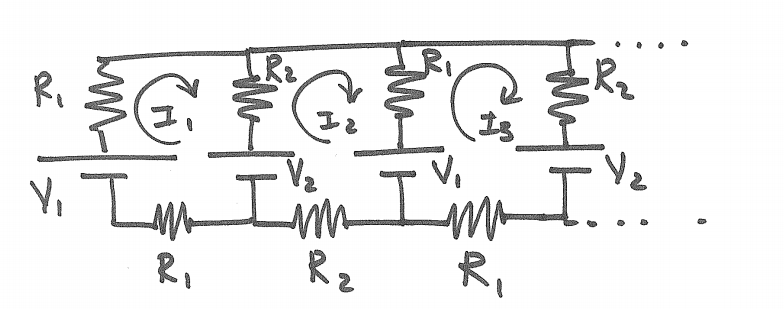
\includegraphics[width=12cm]{circuito.png}
  \caption{\label{fig:circuito} Circuito para el segundo punto.}
\end{figure}

\end{parts}

\end{questions}




\end{document}

